\chapter{Biodiversity}\label{ch:g5:biodiversity}

Take one square metre of flowering meadow and start counting:
a dozen kinds of \omterm{def:g1:plants-around-us:plant}{plants}, beetles and bugs beyond counting,
spiders, snails, worms below and butterflies above. Now try
the same square metre of paved schoolyard. The difference
between those two counts has a name --- \omterm{def:g5:biodiversity:biodiversity}{biodiversity} --- and
it has become one of the most important words in \omterm{def:g1:living-or-not:living}{biology}.

\section{The diversity of life}

\begin{definition}[Species]\label{def:g5:biodiversity:species}
A \emph{species}\index{species} is one particular kind of
\omterm{def:g1:living-or-not:living}{living thing}: all the individuals built on the same model,
which reproduce among themselves. The house sparrow is a
species; so is the common daisy, the red fox, the garden
snail. \Cref{ch:g4:classifying-animals}'s classes are boxes
of many species: ``\omterm{prop:g3:sorting-living-things:groups}{mammals}'' holds thousands of them.
\end{definition}

\begin{definition}[Biodiversity]\label{def:g5:biodiversity:biodiversity}
The \emph{biodiversity}\index{biodiversity} of a place is the
variety of life it holds --- above all, how many different
\emph{\omterm{def:g5:biodiversity:species}{species}} live there, and how well each is doing. A
flowering meadow, rich in \omterm{def:g5:biodiversity:species}{species}, has high biodiversity; a
paved yard, almost none.
\end{definition}

\begin{omfigure}
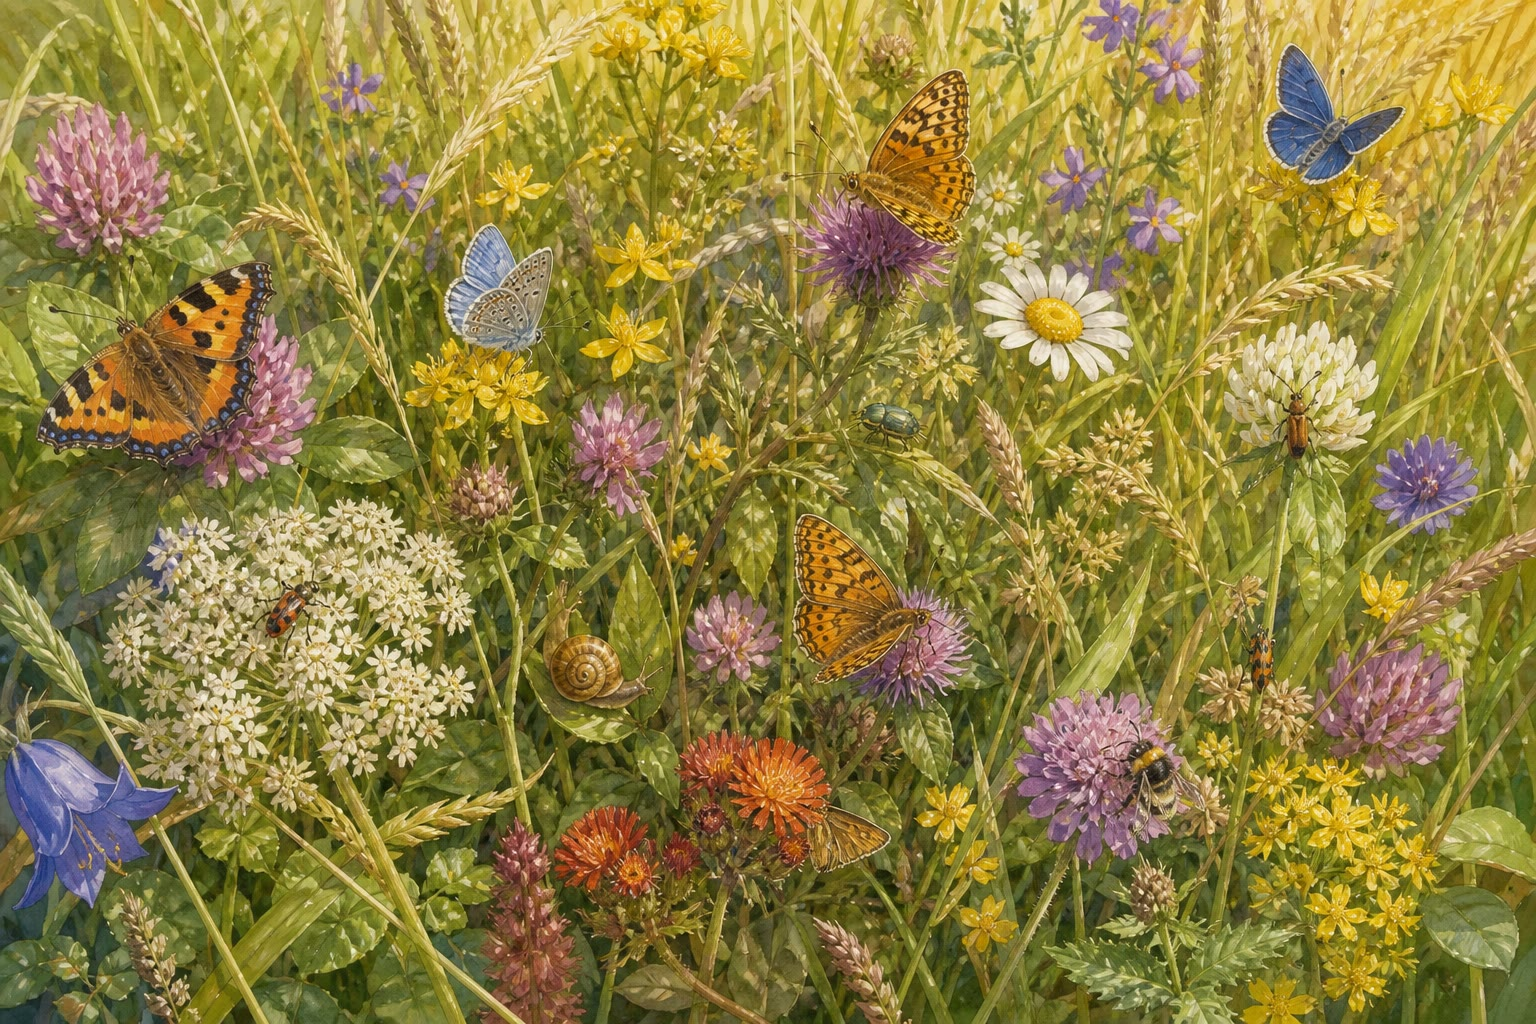
\includegraphics[width=0.62\linewidth]{images/book1/ai/g5-biodiversity-meadow.jpg}

{\small One square metre of meadow, mid-count: grasses,
\omterm{def:g3:flowers-fruits-seeds:parts}{flowers}, butterflies, beetles, a snail --- and the count has
barely begun.}
\end{omfigure}

\begin{example}[Counting the planet]\label{ex:g5:biodiversity:planet}
Scientists have named about two million \omterm{def:g5:biodiversity:species}{species} so far ---
and are sure that is only part of the total, since new
\omterm{def:g5:biodiversity:species}{species} are found on every serious expedition: beetles above
all (no group has more named \omterm{def:g5:biodiversity:species}{species}), but also \omterm{prop:g3:sorting-living-things:groups}{fish}, frogs,
\omterm{def:g1:plants-around-us:plant}{plants}, even occasional \omterm{prop:g3:sorting-living-things:groups}{mammals}. Earth's full \omterm{def:g5:biodiversity:species}{species} count
is still unknown --- most estimates run into the millions
beyond what is named.
\end{example}

\begin{remark}[Diversity at every scale]\label{rem:g5:biodiversity:scales}
\omterm{def:g5:biodiversity:biodiversity}{Biodiversity} shows at several scales at once: many \omterm{def:g5:biodiversity:species}{species} in
one \omterm{def:g2:where-animals-live:habitat}{habitat}; many different \omterm{def:g2:where-animals-live:habitat}{habitats} side by side (pond,
hedge, meadow --- each with its own \omterm{def:g5:biodiversity:species}{species}, as
\cref{ex:g2:where-animals-live:four} showed); and, within one
\omterm{def:g5:biodiversity:species}{species}, no two individuals quite alike --- no two garden
snails wear exactly the same \omterm{def:g1:animals-around-us:covering}{shell}. Variety within variety
within variety.
\end{remark}

\section{Why biodiversity matters}

\begin{proposition}[The web needs its threads]\label{prop:g5:biodiversity:web}
The \omterm{def:g5:biodiversity:species}{species} of a \omterm{def:g2:where-animals-live:habitat}{habitat} feed, shelter, pollinate and clean
up for one another --- they are threads of one web
(\cref{rem:g3:food-chains:web}). A rich web with many threads
can absorb a shock: if one prey \omterm{def:g5:biodiversity:species}{species} fails, its hunters
switch to others. A poor web tears easily: each lost \omterm{def:g5:biodiversity:species}{species}
\omterm{def:g1:plants-around-us:parts}{leaves} the survivors fewer options. \omterm{def:g5:biodiversity:biodiversity}{Biodiversity} is the
web's strength.
\end{proposition}
\admitted

\begin{example}[The orchard test]\label{ex:g5:biodiversity:orchard}
An orchard with hedges, wildflower strips and old trees
hosts dozens of helper \omterm{def:g5:biodiversity:species}{species}: bees and hoverflies
pollinate the blossom
(\cref{rem:g3:flowers-fruits-seeds:bees}), ladybugs eat the
\omterm{def:g1:plants-around-us:plant}{plant} lice, \omterm{prop:g3:sorting-living-things:groups}{birds} patrol for \omterm{ex:g2:animals-grow-up:butterfly}{caterpillars}, worms keep the
soil open. Grub out the hedges and mow the \omterm{def:g3:flowers-fruits-seeds:parts}{flowers}, and the
helpers leave --- the \omterm{prop:g3:flowers-fruits-seeds:transform}{fruit} grower must then do their jobs
alone, jobs the web used to do free.
\end{example}

\begin{example}[People live from the web]\label{ex:g5:biodiversity:people}
Everything humans eat traces back to living \omterm{def:g5:biodiversity:species}{species}
(\cref{rem:g4:what-plants-need:everyone}); most of our
medicines were first found in \omterm{def:g1:plants-around-us:plant}{plants}, molds and other \omterm{def:g1:living-or-not:living}{living
things}; cotton, wool, timber and leather are \omterm{def:g5:biodiversity:species}{species}'
products. The web's threads run straight through every
kitchen, pharmacy and wardrobe.
\end{example}

\section{Biodiversity can be lost --- and helped}

\begin{proposition}[How diversity is lost]\label{prop:g5:biodiversity:loss}
A \omterm{def:g5:biodiversity:species}{species} dwindles when what it depends on is taken:
\begin{itemize}
  \item its \emph{\omterm{def:g2:where-animals-live:habitat}{habitat}} destroyed --- the drained pond of
        \cref{prop:g2:where-animals-live:loss}, the grubbed-out
        hedge, the paved meadow;
  \item its \omterm{def:g2:caring-for-nature:environment}{environment} poisoned --- litter and chemicals
        (\cref{prop:g2:caring-for-nature:harm});
  \item too many of it taken --- overfished, overpicked,
        overhunted.
\end{itemize}
A \omterm{def:g5:biodiversity:species}{species} entirely gone --- everywhere, forever --- is
\emph{extinct}\index{extinct}. Extinction is not like a lost
game: there is no next round.
\end{proposition}
\admitted

\begin{method}[Helping biodiversity, starting small]\label{met:g5:biodiversity:help}
The recipes of \cref{met:g2:caring-for-nature:rules} scale
up:
\begin{enumerate}
  \item keep and \omterm{def:g1:plants-around-us:plant}{plant} variety --- a hedge of five bushes
        beats a fence, a \omterm{def:g3:flowers-fruits-seeds:parts}{flower} strip beats bare gravel;
  \item leave wild corners: dead wood, \omterm{def:g1:plants-around-us:parts}{leaf} piles, unmowed
        grass are \omterm{def:g2:where-animals-live:habitat}{habitats}
        (\cref{ex:g2:caring-for-nature:home});
  \item help the helpers: nest boxes, insect shelters, a
        pond however small
        (\cref{ex:g2:where-animals-live:schoolpond});
  \item count what lives around you, year after year ---
        what is counted is noticed, and what is noticed gets
        protected.
\end{enumerate}
\end{method}

\begin{example}[The return of the storks]\label{ex:g5:biodiversity:storks}
Where wet meadows were restored and nest platforms raised,
storks --- once nearly gone from whole regions --- came back
to breed, and with them frogs, dragonflies and meadow
\omterm{def:g3:flowers-fruits-seeds:parts}{flowers}. \omterm{def:g5:biodiversity:species}{Species} return when their threads are retied:
protection works, and its results can be watched from the
village square.
\end{example}

\section{Exercises}

\begin{exercise}[$\star$]\label{exo:g5:biodiversity:1}
What is a \omterm{def:g5:biodiversity:species}{species}? Give three examples from this chapter.
\end{exercise}

\begin{exercise}[$\star$]\label{exo:g5:biodiversity:2}
What is \omterm{def:g5:biodiversity:biodiversity}{biodiversity}? Compare the meadow and the paved yard.
\end{exercise}

\begin{exercise}[$\star$]\label{exo:g5:biodiversity:3}
About how many \omterm{def:g5:biodiversity:species}{species} are named so far? Why is the true
number certainly higher?
\end{exercise}

\begin{exercise}[$\star$]\label{exo:g5:biodiversity:4}
Name the three scales of diversity in
\cref{rem:g5:biodiversity:scales}, each with its example.
\end{exercise}

\begin{exercise}[$\star$]\label{exo:g5:biodiversity:5}
Why does a species-rich web survive shocks better than a
poor one? Use the hunters-switch-prey argument.
\end{exercise}

\begin{exercise}[$\star$]\label{exo:g5:biodiversity:6}
List four helper \omterm{def:g5:biodiversity:species}{species} of the orchard and the free job
each does.
\end{exercise}

\begin{exercise}[$\star$]\label{exo:g5:biodiversity:7}
Give the three ways a \omterm{def:g5:biodiversity:species}{species} dwindles, with one example
each. What does \emph{\omterm{prop:g5:biodiversity:loss}{extinct}} mean?
\end{exercise}

\begin{exercise}[$\star$]\label{exo:g5:biodiversity:8}
Try it: count the \omterm{def:g5:biodiversity:species}{species} --- \omterm{def:g1:plants-around-us:plant}{plants} and \omterm{def:g1:animals-around-us:animal}{animals}, named or
described --- in one small square you choose outdoors.
Then count a paved square for comparison. Your two numbers
are a \omterm{def:g5:biodiversity:biodiversity}{biodiversity} measurement.
\end{exercise}

\begin{exercise}[$\star\star$]\label{exo:g5:biodiversity:9}
``Losing one beetle \omterm{def:g5:biodiversity:species}{species} out of thousands cannot
matter.'' Answer with
\cref{prop:g5:biodiversity:web} --- and with the fact that
nobody knows all the threads a \omterm{def:g5:biodiversity:species}{species} holds.
\end{exercise}

\begin{exercise}[$\star\star$]\label{exo:g5:biodiversity:10}
The stork story is called a success of \emph{\omterm{def:g2:where-animals-live:habitat}{habitat}}
protection rather than of protecting storks one by one.
Explain the difference, using
\cref{prop:g2:where-animals-live:loss} and what returned
alongside the storks.
\end{exercise}

\begin{exercise}[$\star\star\star$]\label{exo:g5:biodiversity:11}
An orchard keeper replaces hedges and \omterm{def:g3:flowers-fruits-seeds:parts}{flower} strips with
fences and gravel, then must rent beehives for pollination
and spray against \omterm{def:g1:plants-around-us:plant}{plant} lice --- spending money on jobs
once done free. Use \cref{ex:g5:biodiversity:orchard} to
explain what was really removed --- and why the accounts
of nature's free work usually surface only after it stops.
\end{exercise}
